\documentclass[10pt,a4paper]{report}
\usepackage[utf8]{inputenc}
\usepackage{amsmath}
\usepackage{amsfonts}
\usepackage{amssymb}

\usepackage{graphicx}
\author{Helena Brekalo}
\begin{document}

\begin{titlepage}

\newcommand{\HRule}{\rule{\linewidth}{0.5mm}} % Defines a new command for the horizontal lines, change thickness here

\center % Center everything on the page
 
\textsc{\LARGE KU Leuven}\\[1.5cm] % Name of your university/college
\textsc{\Large Ma Ingenieurswetenschappen: Computerwetenschappen}\\[0.5cm] % Major heading such as course name


\HRule \\[0.4cm]
{ \huge \bfseries Development of Secure Software}\\[0.4cm]
\HRule \\[1.5cm]


\textsc{\large Course notes}\\[0.5cm] % Minor heading such as course title


\Large \emph{Author:}\\
Helena \textsc{Brekalo}\\[3cm]

{\large 2015-2016}\\[3cm] % Date

\vfill % Fill the rest of the page with whitespace

\end{titlepage}

\tableofcontents
\clearpage

\chapter{Lesson 1}

\section{Slides: 1. Introduction - Security in Software Development(1)}

Oral exam: 3/4 of the points\\
Project: 1/4 $\rightarrow$ needs to be defended at the exam. Can't be redone in august, grade is kept.

\paragraph{Slide 3-6:} Why is software security so important?
\begin{itemize}
\item Increasing amount of computers: estimated to be at 2 billion 5 years ago. At the moment there are more smartphones than computers and the next wave is that almost all (like IoT) things get internet connectivity these days. This brings its own set of challenges because a PC is different than a car (problems with Jeep!). Much worse things can happen in terms of human safety (pacemakers!). These things pose new threats.
\item There's more and more software. The sizes of the code bases are incredible. A good estimate about the number of bugs is that well-maintained programs have about 100 bugs (I think? -> or 1 bug for every 100 lines). Bugs can become vulnerabilities as soon as they're discovered. The size of the systems is growing every year, OS's get bigger every year. There will never be bug-free systems. 
\item The impact of software grows. Everything runs on software. The important thing is that bugs, 20 years ago, could harm the ICT-industry, now they can harm everything. The yield of cyberweapons is increasing enormously over the past few years. 
\item All the software is more and more connected. We've had software in cars and fridges for years, but it didn't talk to the outside world. Now all these things start talking to each other, getting multiple Internet connections. They become more exposed to possible attacks. It's also seen in the way business is organized: the ordering software of one company may immediately talk to software of another company. It makes things faster and easier, but if there is a bug in there, it may have a bigger impact than when humans are involved.
\end{itemize}

\paragraph{Slide 7:} Definition of computer security: in security we care about the case where we are up against intelligent issues, not issues that may arise randomly. We focus on maintaining some good property in the presence of intelligent adversaries.

\paragraph{Slide 8 a.f.:} Examples of things that have gone wrong:
\begin{itemize}
\item Internet worms and viruses: it's still important today! A worm doesn't need human interaction (can work autonomously). First it was through the exchange of floppy disks, then by requiring human interaction (let people click on images,…). Worms don't need human interaction, that's even "worse" (example: in 30 minutes, the entire world got more infected), they happen even while you're sleeping (Slammer worm) -> completely different concern than human-interactive viruses.
\item Website defacements
\item Jailbreaking or rooting: any device can get jailbroken (the famous ones). Example: 2011 Sony hack, heartbleed (you could specify the length of the payload, but you could make this bigger and the server would provide more than it was actually supposed to send. You couldn't notice it afterwards, but important data could be stolen).
\end{itemize}

\paragraph{Slide 27:}Assets: things that are a value in the system (services, hardware,…).

\paragraph{Slide 28:}Adversary model: in order to reason about security as an engineer, you need to model your adversary. You need to make assumptions about what they can and cannot do. You have to be explicit about what adversaries you worry about.

\paragraph{Slide 29:} You can also start from threats instead of the security goals of your system. Sometimes it makes sense to think about security in the two ways.\\
Threats can be classified (e.g. STRIDE by Microsoft):
\begin{itemize}
\item Spoofing: pretending to be you're someone you're not
\item Tampering: breaking integrity
\item Repudiation: deny having done something that you have done
\item Information disclosure: breaking confidentiality
\item DOS (Denial-Of-Service): flipside of the availability goal
\item Elevation of privileges: expand the access rights you have (you're a student but work as an admin).
\end{itemize}
They're too vague about themselves, you have to be more specific when defining the threats.

\paragraph{Slide 30:} Security argument: you should be able to say that for the security goals that you had in mind/the threats you wanted to counter and under the given adversary model, you can explain that the goals cannot be broken. This is how you defend a security design. It's tricky to get them right because of the intelligent ways of the adversaries.

\paragraph{Slide 31:} Vulnerability: take many forms and enter at many stages (during development, construction or operation).

\paragraph{Slide 32:} Countermeasures: reduce the number of vulnerabilities in the system. They can be preventive, detective or reactive.

\paragraph{Slide 34:} How well the program is documented (and administrated) impacts the security.

\paragraph{Slide 36 a.f.:} Case study: e-mail: divides the internet in a number of domains that have domain names that are familiar. Each of these domains has a number of people that have addresses in these domains and machines that support the system. There are 2 special machines: mail storage server (~pop) and mail transfer server (will route the messages $\rightarrow$ $\sim$smtp). Email (simple version used here): users use the client software to put together the mail and then they'll press 'send' and the mail client will contact the mail transfer server to deliver it. Then the server has the logic to find the right storage server to put the mail in (look at the domain of the recipient and then contact that). If it has a local recipient, then it will immediately hand it over to the ail storage server. Otherwise t will contact the other mail transfer server who will handle the delivery at the appropriate storage server. User 2 then receives the email via its mail client.\\

Potential security goals:
\begin{enumerate}
\item Confidentiality: an email message can only be seen/read by sender and recipient(s).
\item Integrity: modifications to an email message after sending by the sender should be detectable by the recipient.
\item Only users authorized by a domain can send messages from that domain.
\item Only a specific user u at a specific domain d can send messages as u@d.
\item Messages delivered to the system should reach specified recipients' inboxes.
\item Who communicates with whom is confidential.
\item It should be impossible to send viruses to spread through email.
\end{enumerate}
Countermeasures:
\begin{enumerate}
\item Encryption, but where depends: you can encrypt end-to-end or in between.
\end{enumerate}

\chapter{Lesson 2}
Project: reports needed and will be questioned on the exam. 30 hours of (individual) time. 

\section{Slides: 1. Introduction - Security in Software Development(1)}

\paragraph{Slide 40:} We had an analysis of an email system. We didn't pay a lot of attention to what examples of vulnerabilities are. Now we'll talk about vulnerabilities in practice. We'll focus on design and implementation security issues. It's important which vulnerabilities matter the most in practice. 

\paragraph{Slide 41:} The CVE-list is very specific. It identifies a specific vulnerability in a specific version of a specific software product. The CWE tries to abstract a a bit: they define types of threats (e.g. SQL injection, buffer overflow,...) and then classify them according to these types.
It's not based on vulnerabilities that enter early during design! 

\paragraph{Slide 42:} Overview of how important certain vulnerabilities were over a certain stretch. You see types of flaws, then you see over a period of 5 years how common they were (over those 5 years). Then you see for each year specifically how often all the vulnerabilities occurred. 
We'll talk about the top 3. we'll study them in more detail during the course.

\paragraph{Slide 43:} Buffer overflow: make a program misbehave by providing it with some input (exploiting a bug, e.g. writing past the bounds of an array.) If the program doesn't check for that, it will obey and corrupt memory. That may cause the program to overwrite critical data or execute code.

\paragraph{Slide 44:} Typically, on a heavy web application, you have static pages at the web server, business logic at the application server and persistent storage at the back end. There will be code running on the application server. You can write code that dynamically constructs SQL-commands to communicate with the back-end. In SQL-injection you manipulate strings. The given example can be used to check if the user with the given password is registered. If all goes well, then you get the query in \textbf{Slide 46}. the result will contain 1 entry. Otherwise it will send you to a page to create an account. The code is insufficiently defensive.

\paragraph{Slide 47:} If you execute the given code. In SQL, everything after -- is a comment, so it's syntactically correct. The database will ignore the second part, so you can login as user John without entering a password.
Slide 50: related to SQL-injection. Instead of attacking the database, you attack one of the clients. If you know that clients support executional Javascript and if the code is insufficiently defensive, you can send the code at the bottom with a script, which will be sent to the back-end and it will be executed in the client's browser.

\paragraph{Slide 51:} Each of these 3 have to do with input/output validation and defensive coding. If you look at the entire top 10, 80\% of it has to do with this. Bugs in functional parts of the system are more common than other vulnerabilities.\\
We see that vulnerabilities are typically at application-level. They're not in the web server or the OS. In the 90's and before, many attacks were aimed at infrastructure, but since the 2000's, it's more aimed at the applications.

\paragraph{Slide 52:} Vulnerabilities come and go (check the table). It's a moving target. It's not because you're secure against the threats of today, that you'll be safe next year. Security is a process. You can't say "I'm done", that will never happen as long as you're up against an intelligent adversary.

\paragraph{Slide 53:} Top 25 of important threats. Many of them have to do with IO-validation. Some have to do with crypto. The majority has to do with defensive programming.

\paragraph{Slide 54:} Prevalence of vulnerabilities. The blue line seems here to stay. Some vulnerabilities come up and die quickly and are almost not exploited today. The difficult ones only die out very slowly.

\section{Slides: 2. LowLevelSoftwareSecurity}

\paragraph{Slide 1:} For this part, there are good lecture notes! It more or less covers this section of the course (there's a bit more in the slides).

\paragraph{Slide 2:} Implementation-level: bug.

\paragraph{Slide 4:} Memory corruption/safety vulnerabilities: class of vulnerabilities that are relevant for languages that do not check whether programs access memory correctly (e.g. C). 

\paragraph{Slide 5:} There are essentially 4 categories:
\begin{itemize}
\item Spatial safety: program where you declare an array (for example) and you then access it out of bounds. See the first code snippet. The "tenth" access is a spatial safety error. C says that if you declare an array like that, and if you try to access it out of bounds, any correct behaviour is not guaranteed.
\item Accessing: allocate memory and read it before you're assigned to it (I think). It might leak information that was written there before. If you read uninitialized memory, you might read important secrets. It's less risky than the first one, but still important.
\item Temporal: second code snippet: accessing memory after it has been freed. In C memory management is manual. You can then use the memory and manually free it. C says that after you have freed a certain chunk of memory, the behaviour when accessing it is undefined. It's possible that after you freed it, you mess up some important part.
\item Unsafe API: might be that they are unsafe in nature, which you might then exploit. They have a variable number of arguments and you can specify a format string and that way exploit it like spatial safety errors.
\end{itemize}
Java protects against:
\begin{itemize}
\item Spatial safety: you get an exception. It does not leave behaviour undefined. The compiler is forced to check for spatial safety errors
\item Temporal: it does its own garbage collection. There are languages that try to achieve safety without garbage collection, but this is tricky. Something is only freed if you can assure that you can't access it anymore.
\end{itemize}

\paragraph{Slide 6:} C does all this for optimization purposes. C is designed for performance, so that's why it doesn't check bounds etc. If behaviour is undefined, it depends on the compiler: very implementation-dependent. The trick of all attacks will be to know the implementation details so well that you can tune it to your advantage.

\paragraph{Slide 7:} Piece of code with spatial safety vulnerability. The program defines a main function and a cookie, an array of characters. Then you print out the address of the buf-variable and the address of the cookie variable, so you will get the addresses, it helps us exploit it. gets is one of the unsafe C-functions: reads from standard input until it reaches a new line. It will store them in buf. This is where the vulnerability is: it doesn't put a limit on the number of chars it reads, so if you read more than 80, you will have a buffer overflow.\\
Question: how can you make this program print out "you win"? If you add more than 80 chars to buf. Normally cookie and buf will be allocated together on the stack (see Figure \ref{les2_01}). It could also put cookie underneath buf. Compiler chooses this! Assuming the memory grows upwards and you give 80 chars, you start filling the buffer, let it overflow, and then you can write in cookie. Originally, memory was allocated downwards. Modern compilers will sometimes reorder the local variables to make buffer overflows less likely.

\begin{figure}[ht!]
\centering
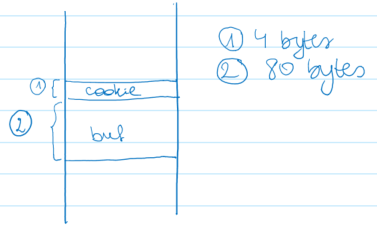
\includegraphics[width=90mm]{Les2_01.png}
\caption{Cookie and buf allocated on the stack together.} 
\label{les2_01}
\end{figure}

\paragraph{Slide 8:} How to make this program print "you win"? Classic stack-based buffer overflow. It's the oldest memory safety issue.

\paragraph{Slide 9:} You can allocate memory in 3 ways:
\begin{itemize}
\item Automatic: you can declare variables in the body of the function. E.g.
\begin{verbatim}
	int f () {
	    int I = 10;
	        char b[80];
	}
\end{verbatim}
Space for these variables will be allocated "automatically": any invocation of f will give you different instantiations of f. when an invocation to f happens, a new part of memory will be allocated on the stack. As a programmer, you don't have to do anything to (de)allocate this. The activation record of the variables will be popped automatically afterwards.
\item Static: it's possible to declare variables outside the body and then you will be able to call it everywhere in the class. The compiler will, once and for all, allocate memory for that variable. You don't have to worry about allocation or freeing because it lives the entire lifetime of the program. E.g.:
\begin{verbatim}
	int j = 10;
	int f () {
	    int I = 10;
	    char b[80];
	}
\end{verbatim}
\item Dynamic: (C: malloc, java: new). This is the only form of explicit memory allocation. Then somewhere in memory, the library will call a piece of memory in runtime until you free it/the garbage collector takes it away. E.g.:
\begin{verbatim}
	int f () {
	    int I = 10;    
	    char b[80];    
	    int * p.malloc(10);
	} 
	free(p);
\end{verbatim}
\end{itemize}

\paragraph{Slide 10:} Division between the data is a convention maintained by the compiler.

\paragraph{Slide 11:} You can see this at work: a program with s a static global variable, a local variable (l) and a dynamic variable (d). See Figure \ref{les2_02}.

\begin{figure}[ht!]
\centering
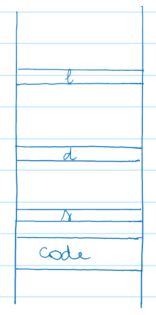
\includegraphics[width=20mm]{Les2_02.png}
\caption{A program with s a static global variable, a local variable (l) and a dynamic variable (d).} 
\label{les2_02}
\end{figure}

\paragraph{Slide 13:} You have a call stack that is used to track function calls and returns. There are local variables and everything that has to do with a specific invocation in the activation record. A consequence is that we have an interesting situation: we have automatically allocated local variables close to other interesting data. If you succeed in finding a bug that overflows the local variables, you don't have to overflow far, you get a lot of power.

\paragraph{Slide 14:} We see the stack and the instruction pointer somewhere in the code (with f1: code for f1). f0 will call f1. On (and on top of) the stack we have an activation record of f0 (if f1 is called within f0). If f0 calls f1, a new activation record is added to the stack. f0 will push the arguments to the stack (\textbf{Slide 15}), then execute the call instruction, this will push the return address on the stack and then, in the entry code of f1, the compiler will emit code that will allocate space for the local variables of f1. After you've finished through the entry code of f1, the entire activation record is on the stack. 
What happens when we overflow? We do something that triggers a spatial memory safety error. The red part in \textbf{Slide 16} is overwritten. You start putting stuff at the bottom of space for buffer \textbf{Slide 15} and then you overwrite all this stuff. How do you overwrite it to be useful to you? The thing to aim for is the return address. If f1 reaches return, the implementation of the machine code will look at that place in the stack and will jump to that part of the machine code, if you overwrite the address, you can do whatever you want. The basic one will overwrite it with an address that is in the stack itself. Because processors don't distinguish between data and code, you can make the processor jump anywhere you want and control this memory content. The stack is the input for the program. You choose the data so that it is interpreted as machine code (I think?). The instruction pointer will go to your instructions and then you can make it do whatever you want.

\paragraph{Slide 17:} Example of a string that when you load it in memory and run it, it will give you an interactive shell. This is extremely machine-specific (OS, processor,…). It's called shell code because that was the main aim of the hackers at the start: to get to the shell.
The infinite loop is to avoid the program from crashing. If you look at the example code (at the top). Our goal is to make the processor execute those 4 bytes (at the left).

\paragraph{Slide 18:} You can address memory at the word level or at the byte level. You can implement that in 2 ways. The addresses go up by 4 because addresses can be accessed by byte or by word. Every one of the words will have 4 bytes associated with it. The choice you make it in what direction you put the bytes (from right to left or from left to right).

\begin{figure}[ht!]
\centering
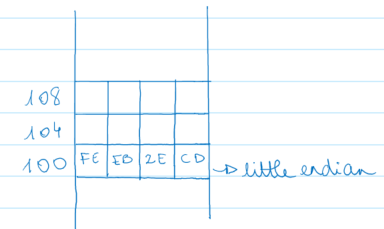
\includegraphics[width=90mm]{Les2_03.png}
\caption{Placement of the attack code.} 
\label{les2_03}
\end{figure}

You can recognize our attack code when you see feeb2ecd: FE EB 2E CD (see Figure \ref{les2_03}). If the processor would be big-endian, you would have to read it the other way around.

\paragraph{Slide 19:} We will attack this program. It takes 2 strings that point to chars. The function allocates a temporary array, then you copy the first string into it and concatenate the second string to it. Then you compare the string to the hardcoded string. If it's equal, you return true, otherwise false. The importance is that the memory safety vulnerabilities are in strcpy and strcat. If the length of either one (or both) of the strings is too large, then you have a buffer overflow. You could implement this with loops too (\textbf{Slide 20}). It does the same thing, but it's harder to see there. 

\paragraph{Slide 21:} We look at the stack right before return. There is room for the tmp array, the saved base pointer, the return address and the 2 arguments. We can see that as we are executing the functions, the different string copies will start copying upward. You see again the little endian at work here (f == 66, I = 69,… -> read the content from right to left). 
We copy the first and the second string: the first string contains 'file' and the second string is the evil one. The code will start to load the second string into the buffer. In \textbf{Slide 22 and 23} we see the tricks at work. \\
At the return address we put chars with the ASCII code that, if we put them in memory, we get the location of our shell code. 

\paragraph{Slide 24:} There's a lot of details to get right. You can't put nulls in your input. If you do that, you are in trouble. The string copy will stop at the null and we won't be able to overflow the buffer. The address we want to jump to contains a null, but we are lucky that it's the last thing we need to overwrite. If it were earlier in the address (say, at the location of ff), the copying would stop early.\\
There are tools that will allow you to tell it to look for certain patterns (like null), and it will look up the machine code to pass it.\\
Nopsled: you look for a string that's big enough and then you start with a -say- 1000 commands that are nop (no operation), then you don't have to aim as precisely as in the other example. Nopsled gives you more "room" to "land". \\
Check out the paper "Smashing the stack for fun and profit"!


\end{document}